\documentclass{article}
\usepackage[german]{babel}
\usepackage[utf8]{inputenc}
\usepackage{tabularx}
\usepackage{listings}
\usepackage{natbib}
\usepackage{graphicx}
\usepackage{url}

\title{Projektbericht TranscriptionDesk}
\author{Robert Rößling, Jakob Runge, Oliver Schurig, Franz Teichmann}
%\date{März 2015}

\begin{document}
%TODO: Stets zwei-drei Sätze Kapiteleinleitung beachten, englische Fachbegriffe auf ein Minimum reduzieren und nicht mehrere Begriffe für eine Semantik nutzen
% z.B. Nutzer statt User, Projekt statt Praktikum

\maketitle

\section*{Abstract}
Lorem ipsum dolor sit amet, consectetur adipiscing elit. Nulla id augue vitae metus blandit tincidunt. In non metus dui. Nunc hendrerit bibendum tellus, vel tempus lorem efficitur id. Quisque ac ex ut felis consectetur sagittis eget et libero. Maecenas eget turpis elit. Ut ex nulla, scelerisque ut tincidunt sit amet, tempor quis risus. Duis blandit posuere tortor lacinia iaculis.

Alle Quelldatein und Installationsanleitungen, usw… gibt es auf GitHub (+ URL, + LICENCE nennen).

\tableofcontents
\newpage
\section{Einleitung}
Im Zuge des Moduls <modul> haben wir dieses studentische Projekt gemacht.

Erläuterung der Dokumentstruktur, aka in diesem Bericht schreiben wir zuerst über <foo>, dann über <bar>.
Später reden wir über <HerpDerp> und letztendlich schließen wir mit <Marderschaden>.
\section{Theoretische Grundlagen}
In diesem Kapitel sollen die Grundlagen für die späteren Erläuterungen gelegt werden. Dazu soll zunächst die Definition von Citizen Science aus der Vorlesung rekapituliert und auf verschiedene Deutungen des Begriffes eingegangen werden, um anschließend eine Arbeitsdefinition für unser Projekt zu geben und es in die Kategorien der Citizen Science nach <Bentham?> einzuordnen. Dazu sei auch auf Literatur zum Thema verwiesen.
\subsection{Definition, Citizen Science}
Zusammenfassung entsprechender Paper + Zitieren.
Unsere Working Definition sollte hier erklärt werden,
und mit anderen Definitionen von Citizen Science verglichen werden.
Zitat von Bentham bietet sich hier an.
\subsection{Kategorien der Citizen Science}
Einordnung unseres Projekts entsprechend der Kategorien für Citizen Science,
wie wir sie in der Vorlesung kennen lernten.
Robert sagt wir sind Dings zwei.
Zitate, wo diese Kategorien her kommen.
\begin{enumerate}
\item foo
\item bar
\item baz
\end{enumerate}
\section{Projektübersicht}
In diesem Kapitel soll eine grundlegende Übersicht über das Projekt und dessen Zielstellung gegeben werden. Dazu soll ausgehend von der Projektvision die Struktur der Datenbasis erläutert und die erwartete Nutzerbasis reflektiert werden.
\subsection{Ziele}
Warum haben wir <herp> gemacht?
Rückbezug zu unserer Definition von Citizen Science.
\subsection{Struktur der Datenbasis}
Wie sehen unsere Dokumente und Rohdaten aus?
Wo kommen diese Daten her?
\subsection{Produkteinsatz / Erwartete Userbasis}
Rückbezug zur Einordnung unserer Software in die entsprechende Kathegorie von Citizen Science.
Warum sollen sich Nutzer registrieren?
\section{Produktfunktion}
Wie können Nutzer an der Seite teilhaben?
Wie registrieren sich Nutzer?
Welche Arbeitsabläufe gibt es?
\section{Architektur}
\subsection{Verwendete Technologien}
LAMP Stack, Browser, JavaScript + Libs, Vagrant, systemd 
Quellen zu den Technologien nennen
\subsection{Gesamtübersicht}
Moduldiagram + Erklärungen
\\\begin{figure}
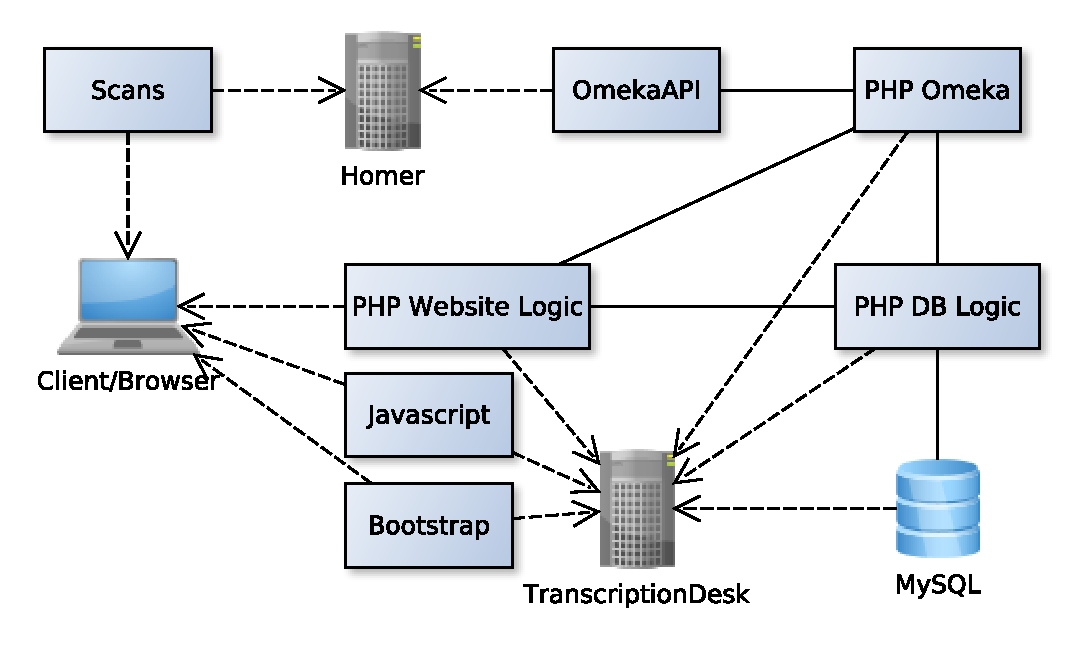
\includegraphics[width=\textwidth]{../notes/components.pdf}
\caption{DESCRIBE ME!}
\label{fig:components}
\end{figure}
\subsection{Datenbank}
ER-Diagram + Erklärungen
\\\begin{figure}
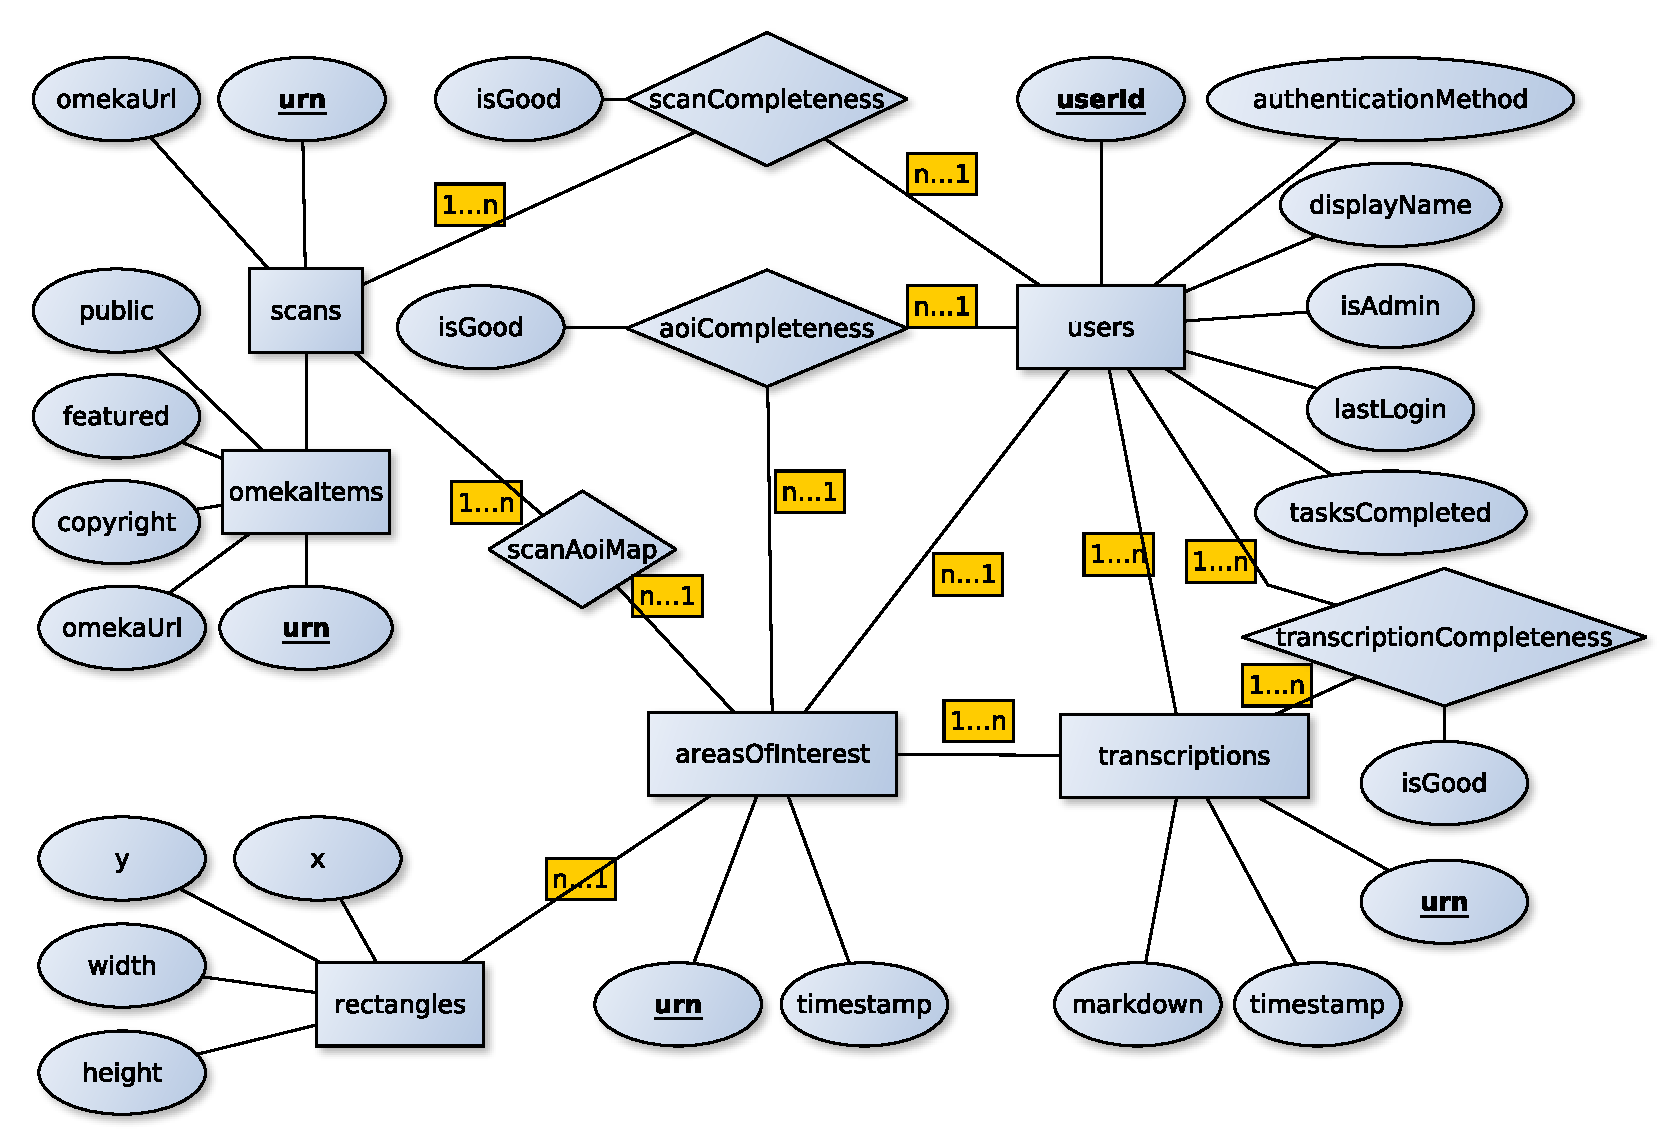
\includegraphics[width=\textwidth]{../notes/ER.pdf}
\caption{DESCRIBE ME!}
\label{fig:er}
\end{figure}
\section{Projektverlauf}
Bisherige Planungsabschnitte,
Entsprechendes Vorgehen unseres Teams,
Entdecken von Issues + Änderungen von Technologieauswahl
Diskussion über URNs
\subsection{Aktueller Stand des Projektes}
\section{Zusammenfassung und Ausblick}
\section*{Quellen}
\bibliographystyle{alpha}
\nocite{*}
\bibliography{references}
\end{document}
